
\documentclass[notheorems,serif]{beamer}

%选用主题
%\usetheme{Rochester}
%\usetheme{default}
%\usetheme{AnnArbor}
%\usetheme{Antibes}
%\usetheme{Bergen}
%\usetheme{Berkeley}
%\usetheme{Berlin}
%\usetheme{Boadilla}
%\usetheme{CambridgeUS}
%\usetheme{Copenhagen}
%\usetheme{Darmstadt}
%\usetheme{Dresden}
%\usetheme{Frankfurt}
%\usetheme{Goettingen}%
%\usetheme{Hannover}
%\usetheme{Ilmenau}
%\usetheme{JuanLesPins}
%\usetheme{Luebeck}
\usetheme{Madrid}
%\usetheme{Malmoe}
%\usetheme{Marburg}
%\usetheme{Montpellier}
%\usetheme{PaloAlto}
%\usetheme{Pittsburgh}
%\usetheme{Rochester}
%\usetheme{Singapore}
%\usetheme{Szeged}
%\usetheme{Warsaw}

% As well as themes, the Beamer class has a number of color themes
% for any slide theme. Uncomment each of these in turn to see how it
% changes the colors of your current slide theme.

%\usecolortheme{albatross}
%\usecolortheme{beaver}
%\usecolortheme{beetle}
%\usecolortheme{crane}
%\usecolortheme{dolphin}
%\usecolortheme{dove}
%\usecolortheme{fly}
%\usecolortheme{lily}
%\usecolortheme{orchid}
%\usecolortheme{rose}
%\usecolortheme{seagull}
%\usecolortheme{seahorse}
%\usecolortheme{whale}
%\usecolortheme{wolverine}

%设置被cover的内容不显示
%\setbeamercovered{transparent}

\useinnertheme{rounded}
\usecolortheme{default}

%调用包
\usepackage[no-math, cm-default]{fontspec}
\usepackage{xltxtra}
\usepackage{xunicode}   
\usepackage{xcolor}
\usepackage{amsmath,amssymb}
\usepackage{xeCJK}
\usepackage{multimedia}
\usepackage{listings}
\usepackage{subfigure}
\usepackage{todonotes}
\presetkeys{todonotes}{inline}{} 
\usepackage{multicol}
\usepackage{changes}




%将系统字体名映射为逻辑字体名称,主要是为了维护的方便  
\newcommand\fnhei{Adobe 黑体 Std}  
\newcommand\fnsong{Adobe 宋体 Std}  
\newcommand\fnkai{Adobe 楷体 Std}  
\newcommand\fnmono{DejaVu Sans Mono}  
\newcommand\fnroman{Times New Roman}  

\renewcommand{\normalsize}{\wuhao}

%%设置常用中文字号,方便调用  
\newcommand{\erhao}{\fontsize{22pt}{\baselineskip}\selectfont}  
\newcommand{\xiaoerhao}{\fontsize{18pt}{\baselineskip}\selectfont}  
\newcommand{\sanhao}{\fontsize{16pt}{\baselineskip}\selectfont}  
\newcommand{\xiaosanhao}{\fontsize{15pt}{\baselineskip}\selectfont}  
\newcommand{\sihao}{\fontsize{14pt}{\baselineskip}\selectfont}  
\newcommand{\xiaosihao}{\fontsize{12pt}{\baselineskip}\selectfont}  
\newcommand{\wuhao}{\fontsize{10.5pt}{\baselineskip}\selectfont}  
\newcommand{\xiaowuhao}{\fontsize{9pt}{\baselineskip}\selectfont}  
\newcommand{\liuhao}{\fontsize{7.5pt}{\baselineskip}\selectfont}  

%\setmainfont{\fnroman}
\setmainfont{\fnkai}
\setCJKmainfont[BoldFont=\fnhei]{\fnkai}  
\setCJKsansfont[BoldFont=\fnhei]{\fnkai}  
\setCJKmonofont{\fnkai}  

%楷体  
%\newfontinstance\KAI{\fnkai}  
%\newcommand{\kai}[1]{{\KAI#1}}  
%黑体  
%\newfontinstance\HEI{\fnhei}  
%\newcommand{\hei}[1]{{\HEI#1}}  
%英文  
%\newfontinstance\ENF{\fnroman}  
%\newcommand{\en}[1]{\,{\ENF#1}\,}

%楷体  
\newfontfamily\KAI {\fnkai}  
\newcommand{\kai}[1]{{\KAI#1}}  
%黑体  
\newfontfamily\HEI{\fnhei}  
\newcommand{\hei}[1]{{\HEI#1}}  
%英文  
\newfontfamily\ENF{\fnroman}  
\newcommand{\en}[1]{\,{\ENF#1}\,}


%连字符
\defaultfontfeatures{Mapping=tex-text}

%中文断行
\XeTeXlinebreaklocale "zh"
\XeTeXlinebreakskip = 0pt plus 1pt minus 0.1pt


%%%% 定理类环境的定义 %%%%
\newtheorem{example}{\hei{例子}} 
\newtheorem{problem}{\hei{问题}}           
\newtheorem{algorithm}{\hei{算法}}
\newtheorem{theorem}{\hei{定理}}
\newtheorem{definition}{\hei{定义}}
\newtheorem{axiom}{\hei{公理}}
\newtheorem{property}{\hei{性质}}
\newtheorem{proposition}{\hei{命题}}
\newtheorem{lemma}{\hei{引理}}
\newtheorem{corollary}{\hei{推论}}
\newtheorem{remark}{\hei{注解}}
\newtheorem{condition}{\hei{条件}}
\newtheorem{conclusion}{\hei{结论}}
\newtheorem{assumption}{\hei{假设}}

%重定义一些环境的名字
\renewcommand{\proofname}{\hei{证明}}
\renewcommand\tablename{\hei{表}}

%---SCRIPT-----------------------------------------------------------------------------------------
\newcommand{\cA}{\mathcal{A}}
\newcommand{\cB}{\mathcal{B}}
\newcommand{\cC}{\mathcal{C}}
\newcommand{\cD}{\mathcal{D}}
\newcommand{\cE}{\mathcal{E}}
\newcommand{\ce}{\mathcal{e}}
\newcommand{\cF}{\mathcal{F}}
\newcommand{\cG}{\mathcal{G}}
\newcommand{\cg}{\mathcal{g}}
\newcommand{\cH}{\mathcal{H}}
\newcommand{\cI}{\mathcal{I}}
\newcommand{\cJ}{\mathcal{J}}
\newcommand{\cK}{\mathcal{K}}
\newcommand{\cL}{\mathcal{L}}
\newcommand{\cM}{\mathcal{M}}
\newcommand{\cN}{\mathcal{N}}
\newcommand{\cO}{\mathcal{O}}
\newcommand{\cP}{\mathcal{P}}
\newcommand{\cQ}{\mathcal{Q}}
\newcommand{\cR}{\mathcal{R}}
\newcommand{\cS}{\mathcal{S}}
\newcommand{\cT}{\mathcal{T}}
\newcommand{\cU}{\mathcal{U}}
\newcommand{\cV}{\mathcal{V}}
\newcommand{\cW}{\mathcal{W}}
\newcommand{\cX}{\mathcal{X}}
\newcommand{\cY}{\mathcal{Y}}
\newcommand{\cZ}{\mathcal{Z}}
\newcommand{\cz}{\mathcal{z}}
%---BLACKBOARD-------------------------------------------------------------------------------------
\newcommand{\mA}{\mathbb A}
\newcommand{\mB}{\mathbb B}
\newcommand{\mC}{\mathbb C}
\newcommand{\mD}{\mathbb D}
\newcommand{\mE}{\mathbb E}
\newcommand{\mF}{\mathbb F}
\newcommand{\mG}{\mathbb G}
\newcommand{\mg}{\mathbb g}
\newcommand{\mH}{\mathbb H}
\newcommand{\mI}{\mathbb I}
\newcommand{\mJ}{\mathbb J}
\newcommand{\mK}{\mathbb K}
\newcommand{\mL}{\mathbb L}
\newcommand{\mM}{\mathbb M}
\newcommand{\mN}{\mathbb N}
\newcommand{\mO}{\mathbb O}
\newcommand{\mP}{\mathbb P}
\newcommand{\mQ}{\mathbb Q}
\newcommand{\mR}{\mathbb R}
\newcommand{\mS}{\mathbb S}
\newcommand{\mT}{\mathbb T}
\newcommand{\mU}{\mathbb U}
\newcommand{\mV}{\mathbb V}
\newcommand{\mW}{\mathbb W}
\newcommand{\mX}{\mathbb X}
\newcommand{\mY}{\mathbb Y}
\newcommand{\mZ}{\mathbb Z}
\newcommand{\mz}{\mathbb z}

\newcommand{\bV}{\mathbf{V}}
\newcommand{\bz}{\mathbf{z}}
\newcommand{\bT}{\mathbf{T}}
\newcommand{\bx}{\mathbf{x}}
\newcommand{\be}{\mathbf{e}}
\newcommand{\bff}{\mathbf{f}}
\newcommand{\bg}{\mathbf{g}}
\newcommand{\bn}{\mathbf{n}}
\newcommand{\bt}{\mathbf{t}}
\newcommand{\bd}{\mathbf{d}}
\newcommand{\bzero}{\mathbf{0}}
\newcommand{\bka}{\mathbf{\kappa}}

\newcommand{\rd}{\mathrm{d}}
%---SHORTCUTS--------------------------------------------------------------------------------------
\newcommand\xor{\mathbin{\char`\^}}
\DeclareMathOperator{\res}{Res}
\DeclareMathOperator{\sgn}{sgn}
\DeclareMathOperator{\supp}{supp}
\DeclareMathOperator{\as}{as}
\newcommand{\slant}[1]{\slshape #1\normalfont}
\newcommand{\dd}[2]{\frac{d#1}{d#2}} 
\newcommand{\ddx}{\frac{d}{dx}}
\newcommand{\ddt}{\frac{d}{dt}}
\newcommand{\dds}{\frac{d}{ds}}
\newcommand{\pd}[1]{\ds\frac{\partial}{\partial #1 }}
\newcommand{\pdd}[2]{\ds\frac{\partial #1}{\partial #2 }}
\newcommand{\mdd}[3]{\ds\frac{\partial^{#3} #1}{\partial #2^{#3} }}
\newcommand{\x}{\ _\Box}
\newcommand{\ds}{\displaystyle}
\newcommand{\bs}{\backslash}
\newcommand{\Bold}{\noindent \bfseries}
\newcommand{\Norm}{\normalfont}
\newcommand{\exl}[1]{\textcolor{NavyBlue}{\Bold Exercise #1 \Norm}}
\newcommand{\ex}{\textcolor{NavyBlue}{\Bold Problem: \Norm}}
\newcommand{\sol}{\textcolor{Mulberry}{\Bold Solution: \Norm}}
\newcommand{\pf}{\textcolor{Mulberry}{\Bold Proof: \Norm}}
\newcommand{\Title}[1]{\LARGE\Bold \textcolor{Sepia}{#1}\Norm\normalsize \vspace{10pt} \newline}
\newcommand{\prop}{\Bold \textcolor{YellowOrange}{ Proposition:} \Norm}
\newcommand{\propl}[1]{\Bold \textcolor{YellowOrange}{ Proposition #1:} \Norm}
\newcommand{\rk}{\Bold \textcolor{YellowOrange}{ Remark:} \Norm}
\newcommand{\rmk}[1]{\Bold\textcolor{YellowOrange}{#1} \Norm}
\newcommand{\thm}[1]{\Bold \textcolor{YellowOrange}{ Theorem #1} \Norm}
\newcommand{\ind}{\indent\indent}
\newcommand{\br}{\vspace{10pt} \newline}

\newcommand{\red}{\color{red}}
\newcommand{\blue}{\color{blue}}



\begin{document}

\title[湘潭大学本科生毕业答辩报告]{{\small\leftline{湘潭大学本科生毕业答辩报告}~~~~~~~~~~~~~~~~~~~~~~~~~~~~~~~~~~~~~~~~~~~~~~
~~~~~~~~~~~} \\
空间分数阶对流扩散方程的有限差分求解
}




\author[周铁军]{~~~报告人:~~周铁军~~ \\
\vspace{0.2cm}
		\qquad\quad\qquad~专~~~~业:~~信息与计算科学~~\\
\vspace{0.2cm}
              \qquad ~~ 导~~~~师:~~文立平 ~教授\\
                }

\institute[湘潭大学数学与计算科学学院]

\date[\today]

\pgfdeclareimage[height=1cm]{institution-logo}{figures/xtu.pdf}

\logo{\pgfuseimage{institution-logo}}


\frame[plain]{\titlepage}


\AtBeginSection[]{

  \frame<beamer>{ 

    \frametitle{内容纲要}   

    \tableofcontents[currentsection] 

  }
}
\section{模型的建立}

\begin{frame}
\frametitle{Lévy-Feller对流-扩散方程的引入}
\qquad Lévy-Feller对流—扩散微分方程:
\begin{equation} 
\frac{\partial u(x, t)}{\partial t}=a D_{\theta}^{\alpha} u(x, t)-b \frac{\partial u(x, t)}{\partial x}
\end{equation}
其中a为正常数,b为常数,算子$D^{\alpha}_{\theta}$表示阶数为$\alpha$、倾斜度为$\theta$的Riesz-Feller分数阶导数。

由文献[5]中的内容可知:
$$D_{\theta}^{\alpha}=-\left[c_{+}(\alpha, \theta) \frac{d^{\alpha}}{d x^{\alpha}}+c_{-}(\alpha, \theta) \frac{d^{\alpha}}{d(-x)^{\alpha}}\right]$$
其中$\frac{d^{\alpha}}{dx^{\alpha}}$和$\frac{d^{\alpha}}{d(-x)^{\alpha}}$分别为左侧和右侧Riemann-Liouville分数阶导数算子。系数c+、c-如下:
\begin{equation*}
\left\{
\begin{aligned}
& c_{+} = c_{+}(\alpha,\theta) := \frac{sin((\alpha-\theta)\pi/2)}{sin(\alpha\pi)}
\\	& c_{-} = c_{-}(\alpha,\theta) := \frac{sin((\alpha+\theta)\pi/2)}{sin(\alpha\pi)}
\end{aligned}
\right.	
\end{equation*}
\end{frame}

\begin{frame}
\frametitle{Lévy-Feller对流-扩散方程的基本解}
\qquad 初边值条件如下:
	\begin{equation*}
	\left\{
	\begin{aligned}
	& u(x, 0)=\varphi(x), \quad (x \in \mathbb{R}) 
	\\	& u( \pm \infty, t)=0, \quad (t>0)
	\end{aligned}
	\right.
	\end{equation*}	
	的Lévy-Feller对流-扩散方程的解析解为
	\begin{equation*}
	\begin{aligned}
	u(x, t) =\frac{1}{2 \pi} \int_{-\infty}^{+\infty+\infty} e^{-i \kappa \xi} e^{t\left(-a|\kappa|^{\alpha} e^{i(s i g n \kappa) \theta \pi / 2}+i b \kappa\right)} \varphi(x-\xi) d \kappa d \xi
	\end{aligned}
	\end{equation*}
\end{frame}


\section{有限区间内的初边值问题}
\begin{frame}
\frametitle{有限区间内的初边值问题的数值解法}
\qquad 给出初边值问题如下:
\begin{equation} 
\begin{array}{ll}{\frac{\partial u(x, t)}{\partial t}=a D_{\theta}^{\alpha} u(x, t)-b \frac{\partial u(x, t)}{\partial x},} & {0<x<R, \quad 0<t<T} \\ {u(x, 0)=\varphi(x),} & {0 \leq x \leq R} \\ {u(0, t)=u(R, t)=0,} & {0 \leq t \leq T}\end{array}
\end{equation}
\end{frame}

\begin{frame}
\frametitle{离散空间与时间变量}
先进行网格剖分,将空间区间[0,L]作M等分,时间区间[0,T]作N等分。其中$h$和$\tau$分别表示空间步长和时间步长,M和N为给定正整数。

利用空间网格点
$$x_{j}=jh,h>0,j=0,\pm1,\pm2,...$$
和时间间隔
$$t_{n}=n\tau,\tau>0,n=0,1,2,...$$
离散空间和时间变量。引入$y_j(t_n):$
$$y_{j}\left(t_{n}\right)=\int_{x_{j}-h / 2}^{x_{j}+h / 2} u\left(x, t_{n}\right) d x \approx h u\left(x_{j}, t_{n}\right)$$
\end{frame}

\begin{frame}
\frametitle{离散空间与时间变量}
\qquad 得到:
\begin{equation}
\frac{\partial u}{\partial t}=\frac{y_{j}\left(t_{n+1}\right)-y_{j}\left(t_{n}\right)}{\tau}+O(t)
\end{equation}
\begin{equation}
\frac{\partial u}{\partial x}=\frac{y_{j}\left(t_{n}\right)-y_{j-1}\left(t_{n}\right)}{h}+O(h)
\end{equation}
以及差分算子$_{h} D_{\theta}^{\alpha}$:

\begin{equation}
_{h} D_{\theta}^{\alpha} y_{j}\left(t_{n}\right)=-\left[c_{+h} D_{+}^{\alpha} y_{j}\left(t_{n}\right)+c_{-h} D_{-}^{\alpha} y_{j}\left(t_{n}\right)\right]
\end{equation}
其中
\begin{equation}
_{h} D_{ \pm}^{\alpha} y_{j}\left(t_{n}\right)=\frac{1}{h^{\alpha}} \sum_{k=0}^{\infty}(-1)^{k} \left( \begin{array}{l}{\alpha} \\ {k}\end{array}\right) y_{j \pm 1 \mp k}\left(t_{n}\right)
\end{equation}
\end{frame}

\begin{frame}
\frametitle{离散空间与时间变量}
\qquad 为了分析算子$_{h} D_{\theta}^{\alpha}$差分格式的收敛性,引入如下引理。
\begin{lemma}
	若函数$u \in L^1(R)$和$H^{\alpha+1}(R)$,$_{h} D_{+}^{\alpha}$为左侧Grünwald-Letnikov分数阶导数算子(或移位算子)的离散:
	\begin{equation}
	_{h} D_{+}^{\alpha} f(x)=\frac{1}{h^{\alpha}} \sum_{k=0}^{\infty}(-1)^{k} \left( \begin{array}{l}{\alpha} \\ {k}\end{array}\right) f(x-(k-p) h)
	\end{equation}
	其中p是一个非负的整数(p=0对应分数阶导数算子,p>0对应移位算子),那么有:当$h \to 0$时,在$x \in R$一致地有:
	\begin{equation}
	_{h} D_{+}^{\alpha} f(x)=_{-\infty} D_{x}^{\alpha} f(x)+O(h)
	\end{equation}
\end{lemma}
\end{frame}

\begin{frame}
\frametitle{离散空间与时间变量}
\qquad 于是原方程表示为:
\begin{equation}
\begin{aligned}
\frac{\boldsymbol{u}_{j}^{n+1}-\boldsymbol{u}_{j}^{n}}{\tau} = & -\frac{\boldsymbol{a}}{\boldsymbol{h}^{\alpha}}\left[\boldsymbol{c}_{+} \sum_{k=0}^{j+1}(-1)^{k} \left( \begin{array}{c}{\alpha} \\ {\boldsymbol{k}}\end{array}\right) \boldsymbol{u}_{j+1-k}^{n}+\boldsymbol{c}_{-} \sum_{k=0}^{N-j+1}(-1)^{k} \left( \begin{array}{c}{\boldsymbol{u}} \\ {\boldsymbol{k}}\end{array}\right) \boldsymbol{u}_{j-1+k}^{n}\right] \\ \\& -\boldsymbol{b} \frac{\boldsymbol{u}_{j}^{n}-\boldsymbol{u}_{j-1}^{n}}{h} + O(t+h)
\end{aligned}
\end{equation}
\qquad 利用边界条件$u_{0}^{n}=u_{N}^{n}=0$,可确定一个线性系统,矩阵形式如下:
\begin{equation*}
U^{\mathrm{n}+1}=A U^{n}
\end{equation*}
其中:
\begin{equation*}
\boldsymbol{U}^{\mathrm{n}+1}=\left(\begin{array}{cccc}{\boldsymbol{u}_{N-1}^{n+1}} & {\boldsymbol{u}_{N-1}^{n+1}} & {\cdots} & {\boldsymbol{u}_{1}^{n+1}}\end{array}\right)^{T}
\end{equation*}
\end{frame}

\begin{frame}
\frametitle{离散空间与时间变量}
\begin{equation*}
\boldsymbol{U}^{\mathrm{n}}=\left( \begin{array}{llll}{\boldsymbol{u}_{N-1}^{n}} & {\boldsymbol{u}_{N-1}^{n}} & {\cdots} & {\boldsymbol{u}_{1}^{n}}\end{array}\right)^{T}
\end{equation*}

而系数矩阵A=(aij)为一个Toeplitz矩阵,	
\begin{equation*}
aij=\left\{
\begin{aligned}
& (-1)^{j-i} \frac{a \tau}{h^{\alpha}} c_{-} \left( \begin{array}{c}{\alpha} \\ {j-i+1}\end{array}\right),
j \geq i+2, i=1,2, \dots, N-3
\\
& -\frac{a T}{h^{\alpha}}\left(c_{+}+c_{-} \left( \begin{array}{l}{\alpha} \\ {2}\end{array}\right)\right),j=i+1, i=1,2, \dots, N-2 
\\
& 1+\frac{a \tau}{h^{\alpha}} \left( \begin{array}{l}{\alpha} \\ {1}\end{array}\right)\left(c_{+}+c_{-}\right)-\frac{b \tau}{h},j=i=1,2, \cdots, N-1 
\\
& -\frac{a \tau}{h^{\alpha}}\left(c_{+} \left( \begin{array}{l}{\alpha} \\ {2}\end{array}\right)+c_{-}\right)+\frac{b \tau}{h},j=i-1, i=2,3, \dots, N-1
\\
& (-1)^{i-j} \frac{a \tau}{h^{\alpha}} c_{+} \left( \begin{array}{c}{\alpha} \\ {i-j+1}\end{array}\right),j \leq i-2, i=3,4, \dots, N-1
\\
\end{aligned}
\right.	
\end{equation*}
\end{frame}


\section{数值实验}

\begin{frame}
    \frametitle{数值算例}
考虑如下Lévy-Feller对流-扩散微分方程初边值问题:
\begin{equation} 
\begin{array}{ll}{\frac{\partial u(x, t)}{\partial t}=a D_{\theta}^{\alpha} u(x, t)-b \frac{\partial u(x, t)}{\partial x},} & {0<x<\pi,\quad 0<t<T}, 1-\alpha \leq 2, \\ {u(x, 0)=\varphi(x)=sin x,} & {0 \leq x \leq \pi,} \\ {u(0, t)=u(R, t)=0,} & {0 \leq t \leq T,}\end{array}
\end{equation}

其中$\alpha$=1.7,$\quad$ $\theta$=0.3,$\quad$ a=1.5,$\quad$ b=1.0.


\end{frame}

\begin{frame}
\frametitle{算法初步}
\begin{table}[h] %开始一个表格environment,表格的位置是h,here。  

	\begin{tabular}{p{2cm}|p{3.5cm}|p{8cm}} %设置了每一列的宽度,强制转换。  
		\hline  
		\hline  
		Step & Operation & Algorithm \\ %用&来分隔单元格的内容 \\表示进入下一行  
		\hline %画一个横线,下面的就都是一样了,这里一共有4行内容  
		one & 网格剖分 & \begin{equation*} 
		\begin{array}{ll}{h=\frac{L}{M},\tau=\frac{T}{N}.} \\ {x=linspace(0,L,M+1);} \\ {t=linspace(0,T,N+1);}\end{array}
		\end{equation*}\\  
		\hline  
		two & 输入初边值 & \begin{equation*} 
		\begin{array}{ll}{u(1:end,1)=\phi(x);} \\ {u(1,1:end)=\psi_{1}(x);} \\ {u(end,1:end)=\psi_{2}(x);}\end{array}
		\end{equation*}\\  
		\hline  
		three & 计算 & \begin{equation*} 
		\begin{array}{ll}{A=Toeplitz(W,V)}\\{for \quad n=1:N} \\ {u(2:end-1,n+1)=A*u(2:end-1,n);} \\ {end}\end{array}
		\end{equation*}\\  
		\hline   
		\hline  
	\end{tabular}  
\end{table}


\end{frame}

\begin{frame}
\frametitle{数值分析}

\qquad 根据上述算法,我们利用MATLAB编程,得到如下图像,并通过plot()函数,直观地表现出u(x,t)的近似程度。
\begin{figure}[h]
	\begin{minipage}[t]{0.4\linewidth}%并排放两张图片,每张占行的0.4,下同 
		\centering     %插入的图片居中表示
		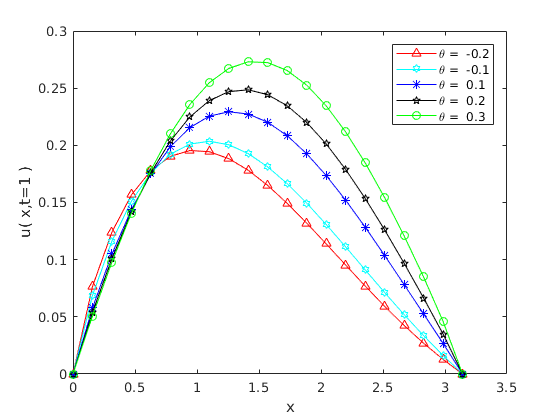
\includegraphics[width=1.2\textwidth]{theta.png}
		\caption{$\theta$取不同值,$\alpha=1.7$时,最后一步数值解的图像}%图片的名称
		\label{fig:liuchengtu1}%标签,用作
	\end{minipage} 
	\hfill
	\begin{minipage}[t]{0.4\linewidth}
		\centering
		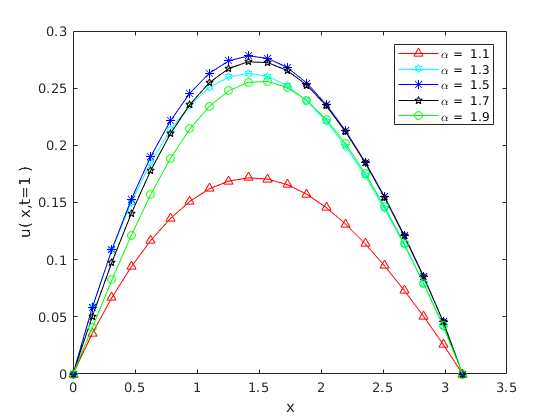
\includegraphics[width=1.2\textwidth]{alpha.png}
		\caption{$\alpha$取不同值,$\theta=0.3$时,最后一步数值解的图像}%图片的名称
		\label{fig:liuchengtu2}
	\end{minipage}
\end{figure}
\end{frame}

\begin{frame}
\frametitle{数值分析}
\begin{figure}[h]
	\begin{minipage}[t]{0.4\linewidth}%并排放两张图片,每张占行的0.4,下同 
		\centering     %插入的图片居中表示
		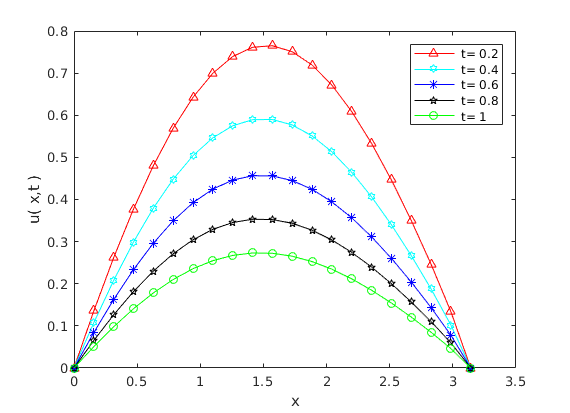
\includegraphics[width=1.2\textwidth]{t1.png}
		\caption{$t$取不同值时,最后一步数值解的图像}%图片的名称
		\label{fig:liuchengtu1}%标签,用作
	\end{minipage} 
	\hfill
	\begin{minipage}[t]{0.4\linewidth}
		\centering
		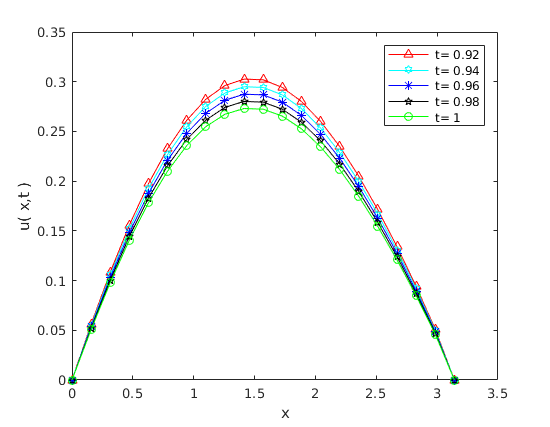
\includegraphics[width=1.2\textwidth]{t2.png}
		\caption{细化t剖分,$t$取不同值时,最后一步数值解的图像}%图片的名称
		\label{fig:liuchengtu2}
	\end{minipage}
\end{figure}
\end{frame}

\begin{frame}
\frametitle{稳定性分析}
我们给初值条件sin(x)加入一个微小干扰,即令$o(h)=\pi/20$,考虑初值条件为sin(x+o(h))时的数值解,得到的图象如下:
\begin{figure}[h]
	\begin{minipage}[t]{0.4\linewidth}%并排放两张图片,每张占行的0.4,下同 
		\centering     %插入的图片居中表示
		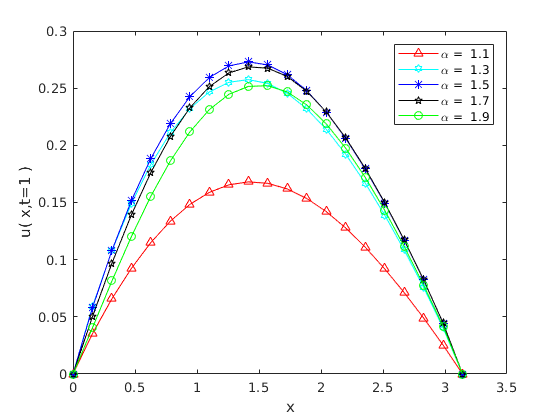
\includegraphics[width=1.2\textwidth]{alpha+o.png}
		\caption{x+o(h)后,$\alpha$取不同值,$\theta=0.3$时,最后一步数值解的图像}%图片的名称
		\label{fig:liuchengtu1}%标签,用作
	\end{minipage} 
	\hfill
	\begin{minipage}[t]{0.4\linewidth}
		\centering
		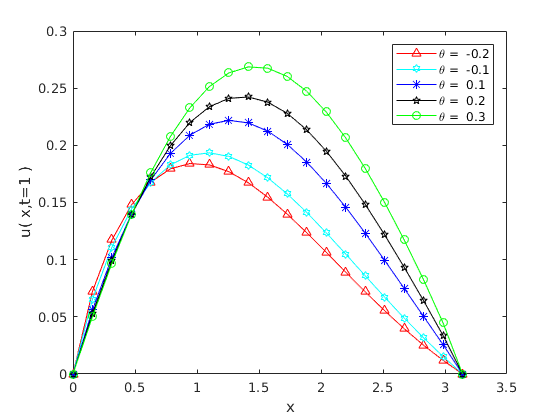
\includegraphics[width=1.2\textwidth]{theta+o.png}
		\caption{x+o(h)后,$\theta$取不同值,$\alpha=1.7$时,最后一步数值解的图像}%图片的名称
		\label{fig:liuchengtu2}
	\end{minipage}
\end{figure}
\end{frame}

\begin{frame}
\frametitle{稳定性分析}
\begin{figure}[h]
	\begin{minipage}[t]{0.4\linewidth}%并排放两张图片,每张占行的0.4,下同 
		\centering     %插入的图片居中表示
		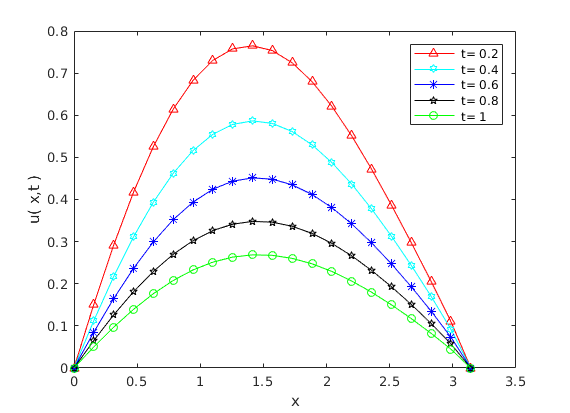
\includegraphics[width=1.2\textwidth]{t1+o.png}
		\caption{x+o(h)后,$t$取不同值时,最后一步数值解的图像}%图片的名称
		\label{fig:liuchengtu1}%标签,用作
	\end{minipage} 
	\hfill
	\begin{minipage}[t]{0.4\linewidth}
		\centering
		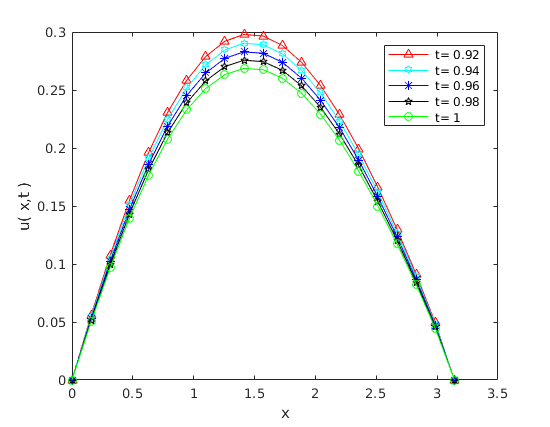
\includegraphics[width=1.2\textwidth]{t2+o.png}
		\caption{细化t剖分,$t$取不同值时,最后一步数值解的图像}%图片的名称
		\label{fig:liuchengtu2}
	\end{minipage}
\end{figure}

通过与初值条件为sin(x)时的图像比较,我们直观地看到其结果的变化是微小的,故我们认为该格式是稳定的。
\end{frame}

\begin{frame}
\frametitle{总结}
\qquad 本文的主要工作是研究的有限区间上的Lévy-Feller对流—扩散方程的初边值问题,进过一系列运算与转化,得到离散的有限差分格式,并利用Matlab对算法进行数值模拟。

通常对于数值模拟问题,人们大多是去讨论解析解与数值解的误差等,对于解析解难求的问题,则无从下手,本文另辟蹊径,讨论了数值解u(x,t)与参数$\theta$,$\alpha$和变量$t$的关系,即对于不同的$\theta$,$\alpha$,$t$,方程的解表现出怎样的形式及特点。

其次,通过不断细化剖分和参数的合理选取,根据函数曲线的收敛情况来分析算法的稳定性、有效性,这也是本文的创新点之所在。
\end{frame}


\section{参考文献}
\setcounter{equation}{0}
\frame{{参考文献}

{\scriptsize
\begin{enumerate}
  \item Liu, Q. and Liu, F. and Turner, I. and Anh, V,
	Approximation of the Lévy–Feller advection–dispersion process by random walk and finite difference method, VOLUME  {222} of {Journal of Computational Physics}PAGES  {57--70},{2007}.
  \item 张贤达,
	矩阵分析与应用[M],
	{北京:清华大学出版社}:{179-197},{2004}.
  \item 王朵,
	{双边空间分数阶对流扩散方程的几种数值解法}, 
	{华南理工大学},{2016}.
  \item 林然,刘发旺,
  分数阶常微分方程初值问题的高阶近似[J],
  {厦门大学学报}{43(1)}:{25--30},{2004}.
  \item 刘青霞,
  {空间分数阶对流-扩散方程的数值解及其应用}, 
  {厦门大学},{2007}.
\end{enumerate}
}
}

\frame{{参考文献}

{
\scriptsize
\begin{enumerate}
\setcounter{enumi}{5}
  \item {段艳婷},
	{二维声波散射正问题的数值解法及应用},
	{西北大学},{2011}.
  \item {祝家麟},
	{边界元方法中的奇异性},
	{土木建筑与环境工程},({2}):{90-102},{1991}.

  \item {李寿佛},
	{刚性常微分方程及刚性泛函微分方程数值分析[M]},
	{湘潭:湘潭大学出版社},{2010}. 
	
  \item {林世敏,许传炬}, 
	{分数阶微分方程的理论和数值方法研究},
	{计算数学},
	{38}({1}):{9--12},{2016}.
  
  \item {林世敏,许传炬}, 
  {数值求解Lévy-Feller扩散方程*},
  {高等学校计算数学学报},
  {27}:{239--241},{2006}.
  
  \item {李荣华},
  {偏微分方程数值解法[M]},
  {北京:科学出版社},{2005}. 
\end{enumerate}
}
}

\begin{frame}
\begin{center}
\Huge \textcolor{red}{谢~~谢~~大~~家!}
\end{center}
\end{frame}

\end{document}
